\subsection{Soft keyboard}

Devices can have hard keyboards or only a directional pad (arrows plus select).

Many of the soft keyboard properties can be set from the device 'Settings'. 

However, \texttt{EditText} views can modify the keyboard using the attribute \texttt{android:inputType}. 
It allows different keys (i.e numeric, email, etc.).

Using the attribute \texttt{android:imeOptions} allows different bottom-right keys instead of 'return'.
Example: Next, Send, Done,...

\subsection{Action Events}

Pressing the bottom-right key raises the \texttt{EditorAction} event.
A listener can be defined in \texttt{EditText} views with \texttt{setOnEditorActionListener()}. 

The bottom right menu is a button to show the keyboard, basically.

You can dismiss the keyboard in the handler. By default, the \texttt{Done} key does that. 
Or you can use the code in the handler:

\begin{lstlisting}[title=Code to hide keyboard]
InputMethodManager mgr = (InputMethodManager) getSystemService(INPUT_METHOD_SERVICE);
mgr.hideSoftInputFromWindow(view.getWindowToken(), 0);
\end{lstlisting}

\subsection{2D graphics on the screen - Canvas}
\hl{To draw in android we use the \texttt{Canvas} API}. Canvas API is a drawing 
framework that is provided in Android, with the help of which we 
can create custom shapes like rectangle, circle, and many more 
in our UI design. 

With the help of this API, we can draw any type of shape for 
our app. The drawing of the different shapes is done using Bitmap. 


\begin{figure}[h]
\centering
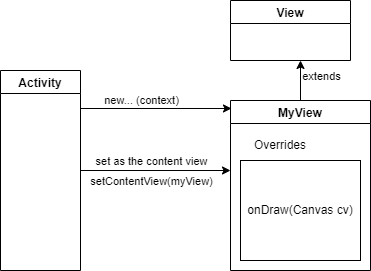
\includegraphics[width=0.7\linewidth]{figures/08_draw_canvas.png}
\caption{Draw Canvas Setup}
\label{fig:draw_canvas}
\end{figure}


The \texttt{Canvas} instance defines a lot of primitives. 
To draw something we use functions like \texttt{draw...}. 
These functions need an instance of \texttt{Paint}. It defines
the characteristics of the drawings, like color, line style and 
width, fonts and sizes, etc. 

Many geometric shapes are defined through a \texttt{Path} instance.
They use the \texttt{canvas.drawPath()} function.

Othre graphic elements are \texttt{Drawable} instances: Bitmaps, 
Shapes, NinePatches, etc. 

Some graphic elements can be defined in xml resources and 
directly used or 'inflated': Colors, Gradients, Shapes, ...


\subsection{Full custom Views}
\hl{This section is mainly an example of how to draw in views.}
Full custom Views need to override several methods from the View
class. 

\begin{itemize}
    \item They can be used in XML layouts;
    \item Parameters from the layout are passed in the
    constructor;
    \item You can create your own event listeners and property
    accessors and modifiers; 
    \item You need to override the \texttt{onMeasure()} method for
    proper behavior, when this View is integrated inside a
    layout; 
    \item You need also to override \texttt{onDraw()} with your
    customized drawing, based on this View properties; 
\end{itemize}

\subsubsection{Example}

\begin{lstlisting}
public class GraphicsView extends View {
    private static final String QUOTE = "Now is the time for all " +
    "good men to come to the aid of their country.";
    private final Path circle;
    private final Paint cPaint;
    private final Paint tPaint;

    public GraphicsView(Context context) {
        super(context);
        circle = new Path();
        circle.addCircle(150, 150, 100, Direction.CW);
        cPaint = new Paint(Paint.ANTI_ALIAS_FLAG);
        cPaint.setStyle(Paint.Style.STROKE);
        cPaint.setColor(Color.LTGRAY);
        cPaint.setStrokeWidth(3);
        tPaint = new Paint(Paint.ANTI_ALIAS_FLAG);
        tPaint.setStyle(Paint.Style.FILL_AND_STROKE);
        tPaint.setColor(Color.BLACK);
        tPaint.setTextSize(20f);
        setBackgroundResource(R.drawable.background);
    }
    @Override
    protected void onDraw(Canvas canvas) {
        canvas.drawPath(circle, cPaint);
        canvas.drawTextOnPath(QUOTE, circle, 0, 20, tPaint);
    }
}
\end{lstlisting}

\begin{lstlisting}
public class Graphics extends Activity {
    @Override
    public void onCreate(Bundle savedInstanceState) {
        super.onCreate(savedInstanceState);
        setContentView(new GraphicsView(this));
    }
}
\end{lstlisting}

\begin{lstlisting}[title=background.xml on res/drawable]
<?xml version="1.0" encoding="utf-8"?>
<shape xmlns:android="http://schemas.android.com/apk/res/android">
<gradient
    android:startColor="#FFFFFF"
    android:endColor="#808080"
    android:angle="270" />
</shape>
\end{lstlisting}

\subsection{Playing audio}
The Android framework encapsulates a complex media player.
Can be used through the framework class \texttt{MediaPlayer}.
\hl{It can work asynchronously} (playing independently of the application) 
and works as a state transition machine object.

Supports a lot of audio formats: wav, aac, mp3, wma, amr (speech), ogg, midi.

For a very simple operation, we must call in order: 
\begin{itemize}
    \item \texttt{release()}: If the object of the MediaPlayer is not null. 
    It is used to release the resources which are associated with MediaPlayer object.
    \item \texttt{create()}: Will create a media player object. We need to specify 
    the resource ID (in res/raw) or a URI: \texttt{mPlayer = MediaPlayer.create(this, R.raw.baitikochi\_chuste);}.
    \item \texttt{start()}: To start playing. It returns immediatly. 
\end{itemize}

\begin{lstlisting}[title=Creates media player on action]
...
@Override
public boolean onKeyDown(int keyCode, KeyEvent event) {
    int resId;
    switch (keyCode) {
        case KeyEvent.KEYCODE_F:
            resId = R.raw.f;
            break;
        default:
            return super.onKeyDown(keyCode, event);
    }

    // Release any resources from previous MediaPlayer
    if (mp != null) {
        mp.release();
    }
    // Create a new MediaPlayer to play this sound
    mp = MediaPlayer.create(this, resId);
    mp.start();
    // Indicate this key was handled
    return true;
}
\end{lstlisting}

\begin{lstlisting}
public class Audio extends Activity {
    private MediaPlayer mp;
    @Override
    public void onCreate(Bundle savedInstanceState) {
        super.onCreate(savedInstanceState);
        setContentView(R.layout.main);
        setVolumeControlStream(
        AudioManager.STREAM_MUSIC);
    }
    ...
}
\end{lstlisting}

\begin{lstlisting}[title=xml]
<LinearLayout xmlns:android=
    "http://schemas.android.com/apk/res/android"
    android:orientation="vertical"
    android:layout_width="fill_parent"
    android:layout_height="fill_parent" >
    <TextView
        android:layout_width="fill_parent"
        android:layout_height="wrap_content"
        android:text="Press the F key"
    />
</LinearLayout>
\end{lstlisting}

\subsection{Playing video}
A video inside a file accessible to your application can be played within a \texttt{VideoView}.

Formats supported include MP4, H.263 (3GP), H.264 (AVC).

Inform the \texttt{VideoView} about the video file path with \texttt{setVideoPath()}.
Start playing with the \texttt{start()} method. 

\hl{Position is not maintained when the device is rotated}. 
Use \texttt{getCurrentPosition()} and save it in \texttt{onSaveInstanceState()}.

Restore the video position with the \texttt{VideoView seekTo()}.

\begin{lstlisting}
public class Video extends Activity {
    @Override
    public void onCreate(Bundle savedInstanceState) {
        super.onCreate(savedInstanceState);
        // Fill view from resource
        setContentView(R.layout.main);
        VideoView video = (VideoView) findViewById(R.id.video);
        // Load and start the movie
        video.setVideoPath("/mnt/sdcard/samplevideo.3gp" );
        video.start();
    }
}
\end{lstlisting}

\begin{lstlisting}[title=XML]
    ...
<FrameLayout
    xmlns:android=
    "http://schemas.android.com/apk/res/android"
    android:layout_width="fill_parent"
    android:layout_height="fill_parent" >
    <VideoView
        android:id="@+id/video"
        android:layout_height="wrap_content"
        android:layout_width="wrap_content"
        android:layout_gravity="center" />
</FrameLayout>

\end{lstlisting}

\begin{lstlisting}[title=Manifest]
...
<activity android:name=".Video"
android:label="@string/app_name"
android:theme=
"@android:style/Theme.NoTitleBar.Fullscreen" >
...
\end{lstlisting}

\subsection{Camera in preview mode}

To display video directly from the camera we need a \texttt{SurfaceView} 
in an \texttt{Activity} layout. 
We need also to orchestrate the camera activation with that \texttt{SurfaceView}
and the \texttt{Activity} life-cycle.

\begin{lstlisting}[title=Steps]
    0. Put a SurfaceView in the Activity layout
    1. [In onCreate()]
    get the SurfaceView from the layout (findViewById())
    get a SurfaceHolder from the SurfaceView (save it on variable)
    add a SurfaceHolder.Callback object (with the callbacks) to the SurfaceHolder
    2. [In onResume()]
    open the Camera (static open() method) and save it
    if the camera was already configured go to 4.
    3. [In the surfaceChanged callback (inside the SurfaceHolder.Callback object)]
    setPreviewDisplay( )
    -- configure the camera
    getParameters()
    -- modify some Parameters
    setParameters()
    4. startPreview() (we see the preview in the screen)
    5. [In onPause()]
    stopPreview()
    release the Camera (release())
\end{lstlisting}


\subsection{3D graphics in Android}

3D graphics are the projection of objects and light on a plane.
The plane is the viewport and is mapped to the screen.

The piece of space projected on the viewport is the
view frustum (a piece of the pyramidal field of view).

\subsubsection{OpenGL}

OpenGL is a big library for 3D graphics programming.
Independent of graphics hardware, designed in 1992 for graphical workstations,
there is a lighter version for mobile devices. 

For using OpenGL ES in Android we use a special view derived from \texttt{GLSurfaceView}.

\begin{figure}[h]
\centering
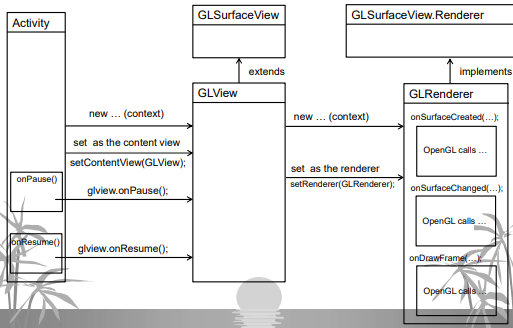
\includegraphics[width=0.8\linewidth]{figures/08_opengl_diagram.png}
\caption{OpenGL diagram}
\label{fig:opengl_diagram}
\end{figure}

% TOUCH EVENTS ========================================================
\subsection{Touch Events}
Many Android devices have only as input the touch screen and gestures.

Many of the events generated by touch are transformed in high level ones like:
\begin{itemize}
    \item Click
    \item LongClick
    \item list item
    \item select
    \item key
\end{itemize}

\hl{But we can intercept them at a lower level using the
\texttt{OnTouchListener} (and its \texttt{onTouch()} method).} 
Since we are in the section about graphics, the touch events 

The \texttt{View} and most of its subclasses generate \texttt{onTouch} events.
Registered with \texttt{setOnTouchListener()}.
When the listener is called it receives the \texttt{View} that caused it and a
\texttt{MotionEvent} instance describing it.

\subsection{MotionEvent}
\texttt{MotionEvent} objects provide information about the touch. 

\begin{itemize}
    \item \texttt{getAction()}: returns in the lower 8 bits a code for theaction: DOWN, UP, MOVE, OUTSIDE, ...
    \item In the higher 8 bits it gives a 'finger' number startingwith 0 (in and after Android 2.2 multitouch issupported).
    \item \texttt{getPointerCount()} returns the number of active 'fingers'.
    \item \texttt{getPointerId(i), getX(i), getY(i)} allows us to extract thenumber and position of each active 'finger'.
\end{itemize}

\begin{lstlisting}[title=Long touch events]
private void dumpEvent(MotionEvent event) {
    String names[] = { "DOWN" , "UP" , "MOVE" , "CANCEL" , "OUTSIDE" ,
    "POINTER_DOWN" , "POINTER_UP" , "7?" , "8?" , "9?" };
    StringBuilder sb = new StringBuilder();
    int action = event.getAction();
    int actionCode = action & MotionEvent.ACTION_MASK;
    sb.append("event ACTION_" ).append(names[actionCode]);
    if (actionCode == MotionEvent.ACTION_POINTER_DOWN || actionCode == MotionEvent.ACTION_POINTER_UP) {
        sb.append("(pid " ).append(action >> MotionEvent.ACTION_POINTER_ID_SHIFT);
        sb.append(")" );
    }
    sb.append("[" );
    for (int i = 0; i < event.getPointerCount(); i++) {
        sb.append("#" ).append(i);
        sb.append("(pid " ).append(
        event.getPointerId(i));
        sb.append(")=" ).append((int) event.getX(i));
        sb.append("," ).append((int) event.getY(i));
        if (i + 1 < event.getPointerCount())
            sb.append(";" );
        }
        sb.append("]" );
        Log.d(TAG, sb.toString());
    }
\end{lstlisting}

\begin{lstlisting}[title=Results]
event ACTION_DOWN[#0(pid 0)=135,179]
event ACTION_MOVE[#0(pid 0)=135,184]
event ACTION_MOVE[#0(pid 0)=144,205]
event ACTION_MOVE[#0(pid 0)=152,227]
event ACTION_POINTER_DOWN(pid 1)[#0(pid 0)=153,230;#1(pid 1)=380,538]
event ACTION_MOVE[#0(pid 0)=153,231;#1(pid 1)=380,538]
event ACTION_MOVE[#0(pid 0)=155,236;#1(pid 1)=364,512]
event ACTION_MOVE[#0(pid 0)=157,240;#1(pid 1)=350,498]
event ACTION_MOVE[#0(pid 0)=158,245;#1(pid 1)=343,494]
event ACTION_POINTER_UP(pid 0)[#0(pid 0)=158,247;#1(pid 1)=336,484]
event ACTION_MOVE[#0(pid 1)=334,481]
event ACTION_MOVE[#0(pid 1)=328,472]
event ACTION_UP[#0(pid 1)=327,471]
\end{lstlisting}


\subsection{Higher level gesteures}

The \texttt{onTouch} listener can pass the \texttt{MotionEventdata} to gesture detectors (Android has two).

\begin{itemize}
    \item \textbf{GestureDetector}: Can detect and trigger events corresponding to one finger gestures.
    Down, Fling, LongPress, Scroll, ShowPress, SingleTap, DoubleTap.
    \item \textbf{ScaleGestureDetector}: Detects the pinch two finger gesture. 
    Generates three events during the gesture: ScaleBegin, Scale, ScaleEnd. 
\end{itemize}


